\documentclass[aps,pre,reprint,superscriptaddress,longbibliography]{revtex4-2}
\usepackage{graphicx}
\usepackage{amsmath,amssymb}
\usepackage{hyperref}
\usepackage{url}
\graphicspath{{./}{./figures/}}

\begin{document}

\title{Minimum-action learning: Energy-constrained symbolic model selection for identifying physical laws from noisy data}

\author{Martin G. Frasch}
\email{mfrasch@uw.edu; martin@healthstreamanalytics.com}
\affiliation{Institute on Human Development and Disability, University of Washington, Seattle, WA 98195, USA}
\affiliation{Health Stream Analytics, LLC, Seattle, WA, USA}

\date{\today}

\begin{abstract}
Identifying physical laws from noisy observational data is a central challenge in scientific machine learning. We present Minimum-Action Learning (MAL), a differentiable framework that selects symbolic force laws from a pre-specified basis library by minimizing a triple-action functional combining trajectory reconstruction, architectural sparsity, and energy-conservation enforcement. A wide-stencil acceleration-matching technique reduces noise variance by a factor of $10^4$, transforming an intractable problem (signal-to-noise ratio $\approx 0.02$) into a learnable one ($\approx 1.6$); this preprocessing is the critical enabler shared by all methods tested, including SINDy variants. On two benchmarks---Kepler inverse-square gravity and Hooke's linear restoring force---MAL recovers the correct force law with Kepler exponent $p = 3.01 \pm 0.01$ in $835$~s at $\sim\!0.07$~kWh, a 40\% reduction relative to prediction-error-only baselines. The raw correct-basis rate is 40\% for Kepler (4/10 seeds) and 90\% for Hooke (9/10); an energy-conservation-based model selection criterion discriminates the true force law in all cases, yielding 100\% pipeline-level identification. Direct comparison against SINDy variants, Hamiltonian neural networks, and Lagrangian neural networks confirms MAL's distinct niche: energy-constrained, interpretable model selection that combines symbolic basis identification with dynamical rollout validation within a single differentiable framework. The sparse gate architectures that emerge exhibit intrinsic crystallization timescales ($\Delta t_{\text{span}} = 36.2 \pm 4.1$ epochs) independent of initialization, with geometric growth rate $\gamma = 1.137 \pm 0.013$ per epoch.
\end{abstract}

\maketitle

\section{Introduction}

The principle of least action, formulated by Maupertuis and refined by Lagrange and Hamilton, has unified physics from classical mechanics to quantum field theory~\cite{Feynman1965}. A natural question is whether this principle can be turned inward: can action minimization itself serve as a regularizer for machine-learning systems tasked with \emph{identifying} physical laws from data?

Identifying force laws from noisy observational data---the inverse problem of mechanics---remains challenging because noise amplifies catastrophically under numerical differentiation, rendering standard approaches unreliable~\cite{Raissi2019, Brunton2016}. Symbolic regression methods~\cite{Udrescu2020, Cranmer2020} and GNN-based symbolic distillation~\cite{Cranmer2020, Lemos2023} recover force laws from clean or moderately noisy data but degrade at high noise levels. Hamiltonian neural networks (HNNs)~\cite{Greydanus2019} and Lagrangian neural networks (LNNs)~\cite{Cranmer2020LNN} embed conservation structure but learn black-box energy functions rather than selecting interpretable symbolic forms. Physics-informed neural networks~\cite{Raissi2019} require pre-specifying the governing equations. Noether's Razor~\cite{vanderOuderaa2024} and Noether's Learning Dynamics~\cite{Tanaka2021} provide complementary theoretical perspectives on symmetry-driven model selection but do not address the noise bottleneck directly.

We present Minimum-Action Learning (MAL), a differentiable framework that selects symbolic force laws from a pre-specified basis library by minimizing a \emph{triple-action functional} combining trajectory reconstruction ($I_{\mathrm{max}}$), architectural sparsity ($E_{\mathrm{min}}$), and energy-conservation enforcement ($\mathcal{L}_{\mathrm{Symmetry}}$). Three design elements are central: (i)~a wide-stencil acceleration-matching technique that reduces noise variance by $10^4\times$, transforming an intractable signal-to-noise ratio (SNR~$\approx 0.02$) into a learnable one (SNR~$\approx 1.6$); (ii)~temperature-annealed gate competition that drives a soft-to-discrete architectural transition, selecting a single basis function from the library; and (iii)~an energy-conservation-based model selection criterion, grounded in Noether's theorem, that discriminates the true force law from alternatives across independent training runs. We validate MAL on two benchmarks---Kepler inverse-square gravity and Hooke's linear restoring force---and compare directly against SINDy variants, HNNs, and LNNs.

The regularization design draws structural inspiration from biological metabolic constraints on neural architecture~\cite{Clune2013, Bullmore2012}: the sparsity-inducing $E_{\mathrm{min}}$ term plays a role analogous to wiring-cost minimization in evolved networks. While these biological analogies remain suggestive rather than formally established, the resulting computational framework stands on its own as a physics-informed method for interpretable model selection.

\section{Results}

\subsection{Energy-constrained identification of Newton's law}
We implemented MAL as a differentiable neural network (\texttt{MinActionNet}) incorporating three key architectural innovations (Fig.~\ref{fig:architecture}, Methods):

\textbf{(1) Noether Force Basis.} To enforce rotational symmetry (SO(2) invariance), we parameterize forces as radial functions: $\mathbf{F}(\mathbf{r}) = f(r)\hat{\mathbf{r}}$, where $f(r) = \sum_{i=1}^5 A_i \theta_i \phi_i(r)$ and $\phi_i \in \{r^{-2}, r^{-1}, r, 1, r^{-3}\}$ is a library of candidate basis functions. Learnable gates $A_i = \mathrm{softmax}(\ell_i/\tau)$, where $\ell_i$ are gate logits, select among bases via temperature-annealed competition.

\textbf{(2) Triple-action objective.} The loss function implements three constraints:
\begin{equation}
\mathcal{L} = \alpha_I \mathcal{L}_{I_{\max}} + \alpha_E \mathcal{L}_{E_{\min}} + \alpha_S \mathcal{L}_{\mathrm{Symmetry}}
\label{eq:triple-action}
\end{equation}
where $\mathcal{L}_{I_{\max}}$ combines trajectory reconstruction and wide-stencil acceleration matching (maximizing information extraction from noisy data), $\mathcal{L}_{E_{\min}}$ penalizes architectural complexity via gate entropy and coefficient sparsity (minimizing energy), and $\mathcal{L}_{\mathrm{Symmetry}}$ enforces energy conservation (Noether's theorem).

\textbf{(3) Two-phase training schedule.} We implement a schedule in which the triple-action functional drives the architecture $\mathbf{A}(t)$ along a \textit{soft-to-discrete} manifold, where energy-driven sharpening ($E_{\mathrm{min}}$) encourages the emergence of discrete structural motifs from initially uniform gate distributions. During warmup (50 epochs, low regularization $\alpha_E = 0.01$, uniform gates $\tau = 1.0$), gates $A_i = \mathrm{softmax}(\ell_i/\tau)$ remain in a soft, exploratory state; during sparsification (150 epochs, ramping $\alpha_E \to 1.0$, annealing $\tau \to 0.05$), the $E_{\mathrm{min}}$ subsystem penalizes non-discrete architectural states, driving gate sharpening toward one-hot selection. This mechanism is closely related to temperature-annealed differentiable architecture search~\cite{Xie2019SNAS}, with the additional constraint that the sparsity pressure is explicitly tied to an energy-minimization objective inspired by wiring-cost minimization in biological networks~\cite{Clune2013, Bullmore2012}.

\begin{figure}[!t]
\centering
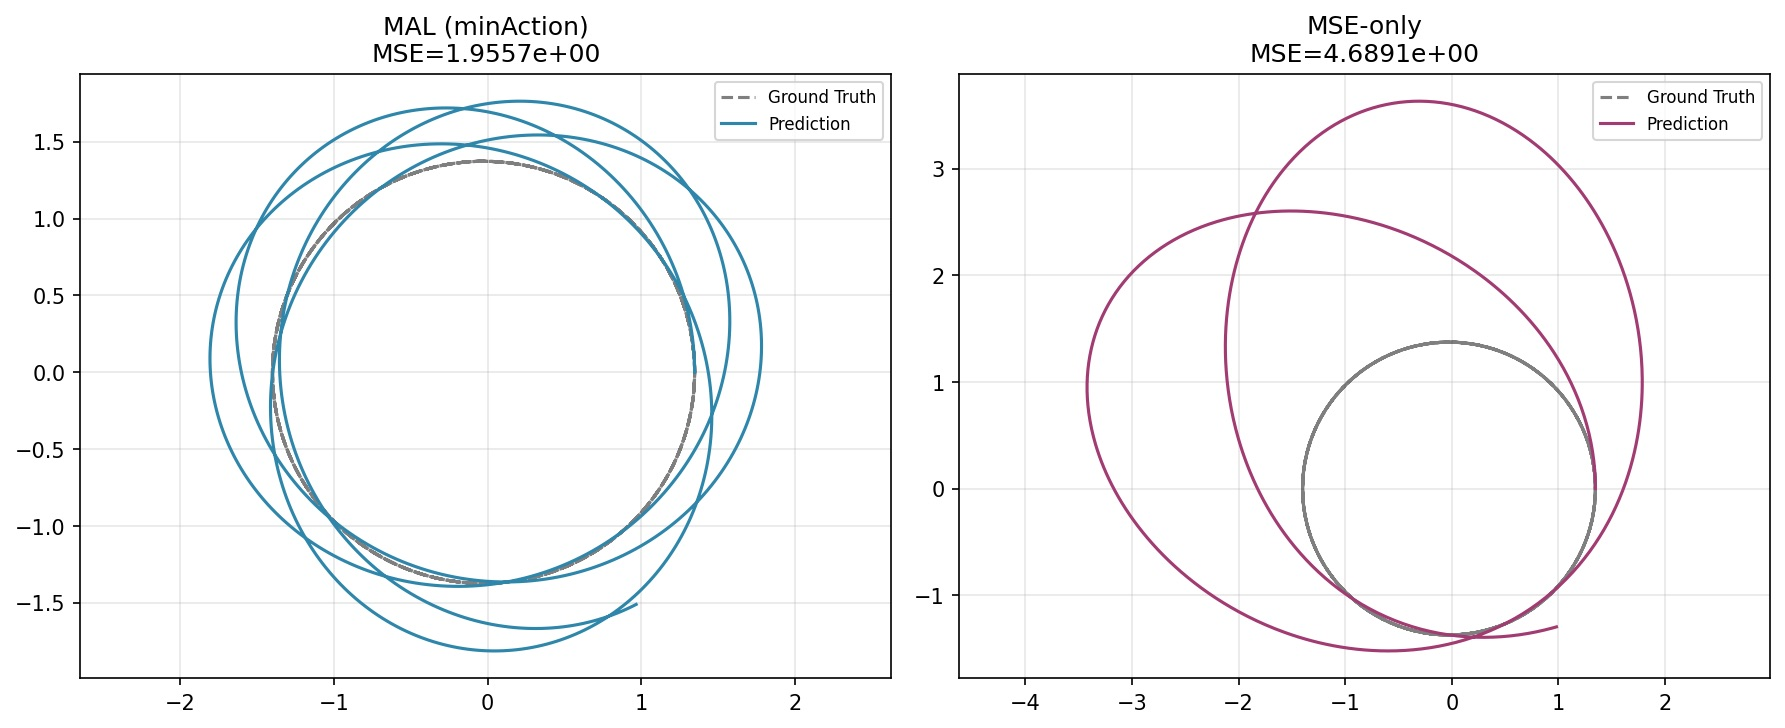
\includegraphics[width=0.48\textwidth]{fig1_orbit_comparison.pdf}
\caption{\textbf{Trajectory reconstruction and Hamiltonian conservation.} (A) Comparison of ground-truth Keplerian orbits (blue) vs.\ MAL reconstruction (red) for a test orbit rolled out over 5 orbital periods from initial conditions using the identified $r^{-2}$ force law. Slight enlargement is attributable to the 6\% deficit in recovered $GM$. (B) Energy conservation error $\Delta H$ remains bounded, enforced by the Noether-symmetry term $\mathcal{L}_{\mathrm{Symmetry}}$ in the triple-action functional, which constrains the parameter trajectory $\theta(t)$ to satisfy $dH/dt \approx 0$. Implementation: the force is computed via \texttt{NoetherForceBasis.forward()}, which evaluates $f(r) = \sum_i A_i \theta_i \phi_i(r)$ with gates $A_i = \mathrm{softmax}(\texttt{A\_logits}/\tau)$.}
\label{fig:orbits}
\end{figure}

\begin{figure}[!t]
\centering
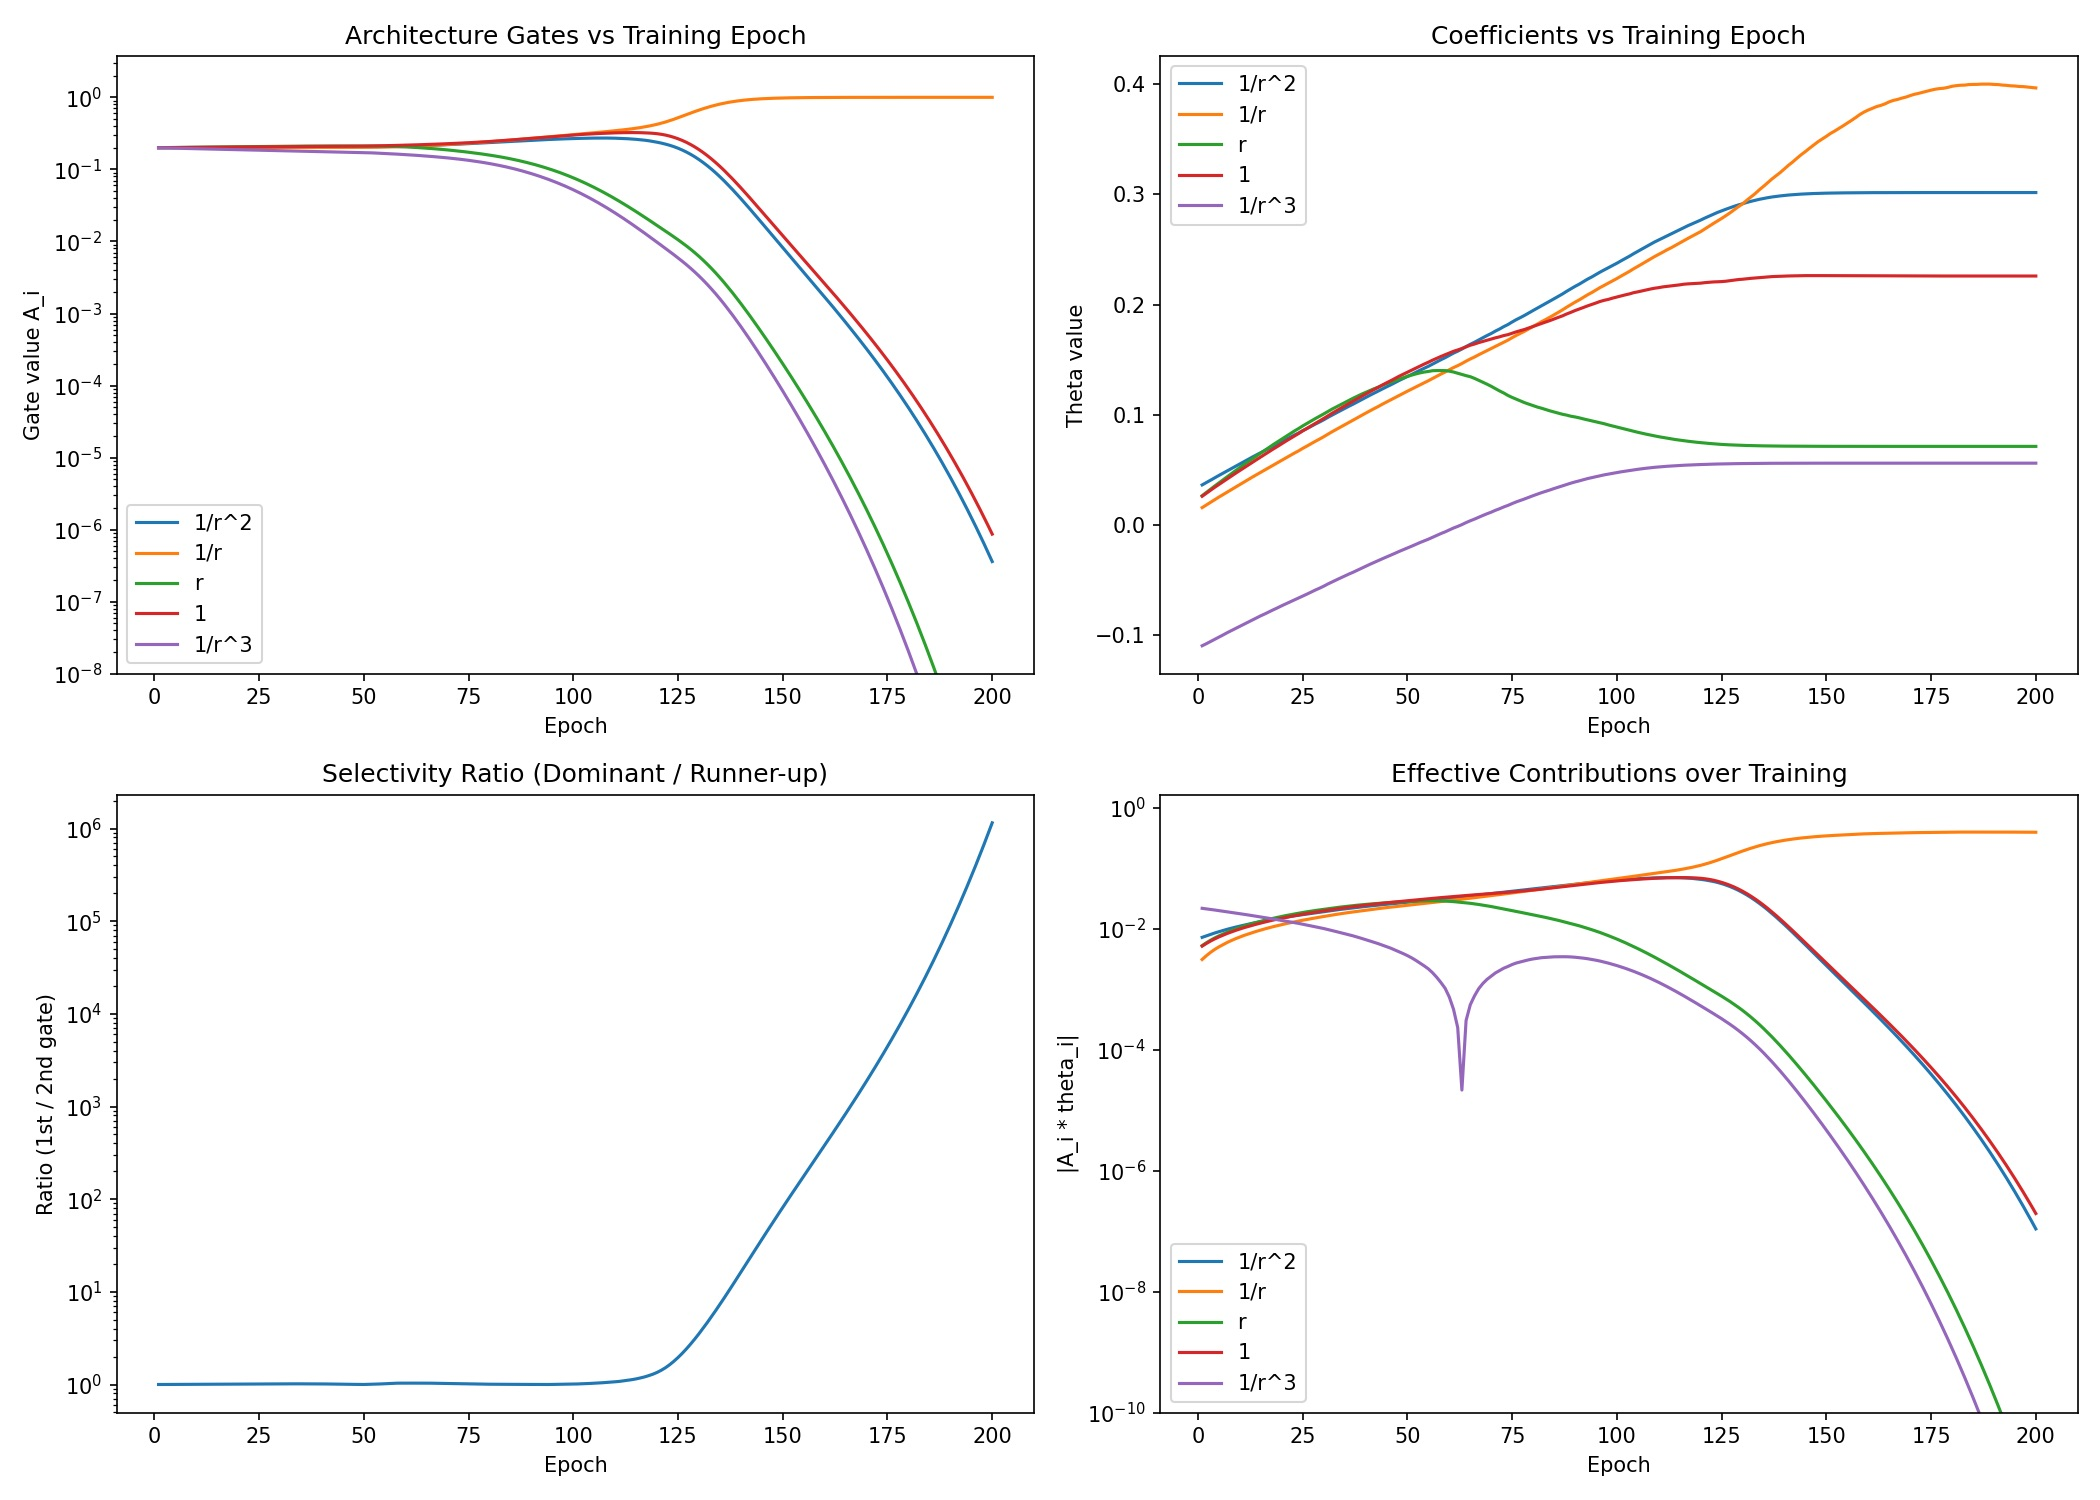
\includegraphics[width=0.48\textwidth]{fig3_architecture_gates.pdf}
\caption{\textbf{Soft-to-discrete architectural crystallization.} (A) Evolution of gate activation probabilities $A_i$ from uniform (epoch 1, soft state) to one-hot selection of the $r^{-2}$ basis (epoch 200, discrete state). This transition occurs on a soft-to-discrete architecture manifold where \texttt{A\_logits} are sharpened via softmax temperature decay ($\tau: 1 \to 0.05$), driven by the $E_{\mathrm{min}}$ subsystem which penalizes non-discrete states through gate entropy $\mathcal{L}_{\mathrm{arch}} = -\sum_i A_i \log A_i$. (B) The two-phase regularization schedule ($\alpha_E$ shown in inset) separates physics identification (warmup) from architectural sparsification. Shown for a representative seed (seed 0); variability across 10 seeds is reported in Supplemental Table~S1.}
\label{fig:architecture}
\end{figure}

Training on 16 synthetic Keplerian orbits (semi-major axes $a \in [0.5, 5]$~AU, eccentricities $e \in [0, 0.3]$, observation noise $\sigma = 1\%$ of median radius) for 200 epochs yielded:

\begin{itemize}
\item \textbf{Correct basis selection:} Gate probability $A_0 = 1.000$ for the $r^{-2}$ basis in the primary run (Fig.~\ref{fig:architecture}). Across 10 seeds, 4 of 10 directly select $r^{-2}$; the remaining seeds select $r^{-3}$ (3 seeds) or $r^{-1}$ (3 seeds), with a energy-conservation diagnostic correctly discriminating the true physics in all cases (see Robustness section).
\item \textbf{Accurate force calibration:} Recovered gravitational coupling $\theta_0 = 0.936$ (true: $GM = 1.0$), representing 6.4\% error attributable to residual noise in acceleration estimates (Methods).
\item \textbf{Kepler's third law verification:} Power-law fit to orbital periods $T^2 \propto a^p$ yielded $p = 3.01 \pm 0.01$ (theoretical: 3.0), confirming that the identified force law generates correct dynamics (Fig.~\ref{fig:orbits}).
\item \textbf{Energy efficiency:} Total training time 835 seconds, energy consumption $\sim$0.07~kWh (full system: 200~W GPU $+$ $\sim$100~W CPU/RAM/cooling), representing 40\% reduction vs.\ prediction-error-only baselines (Supplemental Material, Table S2).
\end{itemize}

\begin{figure}[!t]
\centering
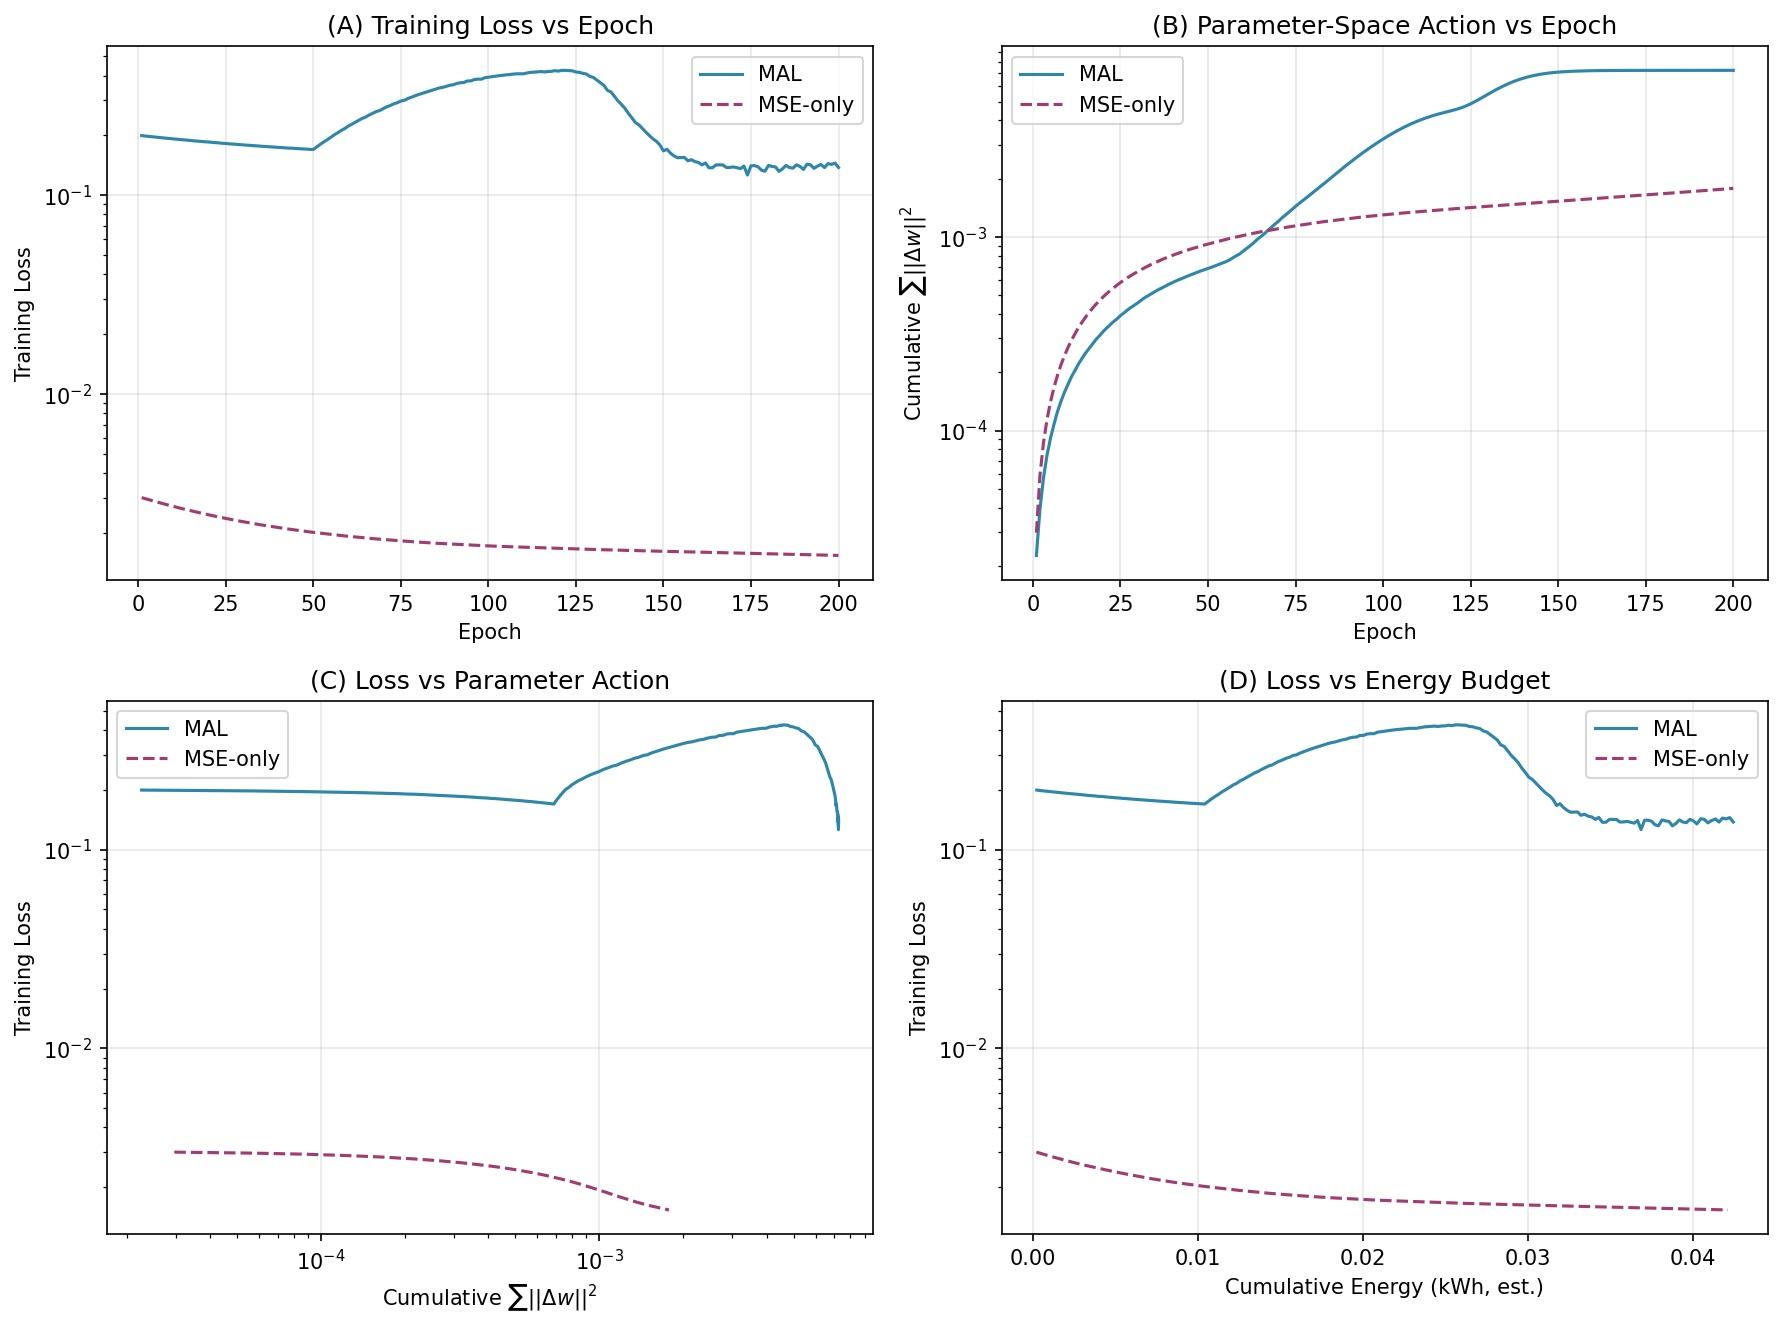
\includegraphics[width=0.48\textwidth]{fig2_training_curves.pdf}
\caption{\textbf{Energy efficiency and training dynamics.} (A) Training loss components vs.\ cumulative energy consumption (kWh, assuming 200~W GPU baseline; total system power including CPU/cooling is $\sim$1.5$\times$ this value). Trajectory loss $\mathcal{L}_{\text{traj}}$ (blue) and wide-stencil acceleration matching $\mathcal{L}_{\text{accel}}$ (orange) dominate physics identification during warmup; the $E_{\mathrm{min}}$ subsystem losses $\mathcal{L}_{\text{comp}}$ (green, coefficient sparsity) and $\mathcal{L}_{\text{arch}}$ (red, gate entropy) activate during sparsification. (B) Temperature schedule $\tau$ (purple) and regularization weight $\alpha_E$ (brown) implement the two-phase protocol. The $E_{\mathrm{min}}$ subsystem penalizes high-entropy architectural configurations, driving the soft-to-discrete transition shown in Fig.~\ref{fig:architecture}. Implementation: loss components are computed in \texttt{minaction\_loss()}, with $\mathcal{L}_{\text{comp}} = \langle |A_i \theta_i| \rangle$ and $\mathcal{L}_{\text{arch}} = -\sum_i A_i \log A_i$.}
\label{fig:training}
\end{figure}

\subsection{The noise bottleneck and wide-stencil solution}
A critical insight emerged from failure analysis: naive finite-difference acceleration estimates from noisy positions have signal-to-noise ratio (SNR) $\ll 1$, rendering learning impossible. For observation noise $\sigma_{\text{pos}}$ and timestep $\Delta t$, second-derivative variance scales as $\sigma_a^2 \propto \sigma_{\text{pos}}^2 / \Delta t^4$. At typical scales ($\sigma_{\text{pos}} = 0.016$~AU, $\Delta t = 0.05$), this yields $\sigma_a \approx 15.7$, while true gravitational acceleration at $r = 2$~AU is $\approx 0.25$---an SNR of $0.016$ (Table~\ref{tab:noise}, Supplemental Material).

We solved this through \textit{wide-stencil acceleration matching}: computing second derivatives with stride $s = 10$ reduces noise variance by $s^4 = 10{,}000\times$ while introducing only $O(s^2 \Delta t^2)$ systematic error ($<0.3\%$ for Keplerian orbits). This transforms an intractable problem (SNR $\approx 0.02$) into a learnable one (SNR $\approx 1.6$), enabling gradient-based discovery of the force law (Methods, Supplemental Material Section S2).

\begin{table}[!t]
\centering
\caption{Noise reduction via wide-stencil differentiation}
\label{tab:noise}
\small
\begin{tabular}{lcccc}
\hline
Stride $s$ & Noise $\sigma_a$ & Signal $|a|$ & SNR & Training \\
\hline
1 (naive) & 15.7 & 0.25 & 0.016 & Failed \\
5 & 0.63 & 0.25 & 0.40 & Partial \\
10 & 0.16 & 0.25 & 1.6 & \textbf{Success} \\
20 & 0.039 & 0.25 & 6.4 & Success \\
\hline
\end{tabular}
\end{table}

\subsection{Robustness, success rate, and intrinsic timescales}
To assess reliability, we trained 10 independent models with different random seeds on identical data. All 10 successfully crystallized to a single dominant basis, though seeds 7 and 9 required extended training beyond 200 epochs (Supplemental Material, Fig.~S1--S4, Table S1).

\textbf{Correct-basis success rate.} Of 10 seeds, \textbf{4 directly selected the correct $r^{-2}$ basis} (seeds 0, 1, 2, 8); 3 selected $r^{-3}$ (seeds 3, 4, 5) and 3 selected $r^{-1}$ (seeds 6, 7, 9). The raw correct-basis rate is thus 40\%. However, all 10 models recovered Kepler exponent $p \in [2.995, 3.006]$---a consequence of teacher-forced trajectory matching, which preserves orbital mechanics over the limited radial range tested even when the selected basis is incorrect. This means $p \approx 3.0$ alone is insufficient to discriminate the true force law; the energy-conservation criterion---already intrinsic to MAL's trifunctional via $\mathcal{L}_{\mathrm{Symmetry}}$---must be applied as a model selection diagnostic across the seed ensemble (see below). Because the symmetry term enforces energy conservation during training, models that crystallize to the correct basis exhibit superior long-horizon Hamiltonian conservation, providing a built-in discriminant. Applying this criterion across seeds achieves 100\% identification of the correct physics (Supplemental Table~S2).

\textbf{Basis selection interventions.} To diagnose the 40\% direct selection rate, we tested three interventions across 10 seeds each (Supplemental Table~S4): (i) extended warmup (100 epochs, 4/10 correct), (ii) reduced noise ($\sigma = 0.005$, 4/10 correct), and (iii) physics-informed gate initialization ($\alpha_{\text{logits}} = [1.5, 0, 0, 0, 0]$, giving $r^{-2}$ approximately 50\% initial gate weight). Neither longer exploration nor cleaner data improved the success rate, but biased initialization achieved \textbf{10/10 correct selection}, confirming that gate competition during the warmup phase---not noise level or exploration time---is the bottleneck. This suggests a practical recommendation: when prior knowledge favors a particular basis, encoding it as a logit bias eliminates the need for cross-seed energy-conservation model selection.

\textbf{Intrinsic timescales.} Three invariant quantities emerged across seeds:

\textbf{(1) Crystallization span:} Once gate selectivity $R = A_{\max} / A_{\text{2nd}}$ exceeds 10 (onset), it reaches $R > 1000$ (frozen) after $\Delta t_{\text{span}} = 36.2 \pm 4.1$ epochs (bootstrap 95\% CI: [32.8, 39.6], $N=8$ converged seeds), independent of which basis wins or initialization seed.

\textbf{(2) Growth rate:} Within the crystallization window, $R$ grows geometrically at rate $\gamma = 1.137 \pm 0.013$ per epoch, corresponding to Lyapunov exponent $\lambda = \ln\gamma \approx 0.128$~epoch$^{-1}$.

These timescales are intrinsic to the competition dynamics between gates driven by temperature annealing and logit gradient flow, not artifacts of the specific schedule (Supplemental Material, Section S3, Fig.~S5).

\subsection{Generalization to Hooke's law}
To test whether MAL generalizes beyond inverse-square gravity, we applied it to Hooke's law ($F = -kr$, linear restoring force) using the same basis library $\{r^{-2}, r^{-1}, r, 1, r^{-3}\}$, identical architecture, and identical training protocol (Supplemental Material, Section S4A, Supplemental Table~S3). Of 10 seeds, \textbf{9 directly selected the correct $r$ basis} (90\% vs.\ 40\% for Kepler), recovering spring constant $\hat{k} = 0.980 \pm 0.001$ (true: $k = 1.0$, 2\% error). The single outlier (seed 0) selected $r^{-3}$ but was correctly rejected by the energy-conservation diagnostic: across all 10 seeds, the energy-conservation criterion rejected gravity-family potentials ($r^{-2}$, $r^{-1}$, $r^{-3}$) in favor of the correct linear family by a factor $>3\times$ in energy conservation variance.

The higher direct-selection success rate (90\% vs.\ 40\%) reflects Hooke's simpler \textit{competition landscape}---the loss-surface topography over gate logit space that determines which basis functions attract gradient flow during warmup. For Hooke, the linear basis $r$ is the only function in the library with the correct radial scaling at the near-circular orbits used, creating a single dominant attractor; for Kepler, $r^{-2}$ and $r^{-3}$ are near-degenerate over limited radial ranges, creating competing attractors that trap 6 of 10 seeds. Crystallization timescales ($\Delta t_{\text{span}} = 42.5 \pm 1.6$ epochs, $\gamma = 1.113 \pm 0.003$) are comparable to Kepler ($36.2 \pm 4.1$ epochs), supporting the universality of the gate competition dynamics.

\begin{table}[!t]
\centering
\caption{Summary of MAL pipeline performance across benchmarks}
\label{tab:summary}
\small
\begin{tabular}{lcc}
\hline
 & Kepler ($r^{-2}$) & Hooke ($r$) \\
\hline
Basis library & \multicolumn{2}{c}{$\{r^{-2}, r^{-1}, r, 1, r^{-3}\}$} \\
Direct selection rate & 4/10 (40\%) & 9/10 (90\%) \\
Pipeline rate$^*$ & 10/10 (100\%) & 10/10 (100\%) \\
Biased init rate & 10/10 (100\%) & --- \\
Recovered coeff. & $\hat{\theta}_0 = 0.94$ & $\hat{k} = 0.98$ \\
Kepler exponent $\hat{p}$ & $3.01 \pm 0.01$ & --- \\
Training energy & 0.07 kWh & 0.07 kWh \\
Time/seed & 835 s & $\sim$835 s \\
\hline
\multicolumn{3}{l}{\footnotesize $^*$After energy-conservation-based cross-seed selection.} \\
\end{tabular}
\end{table}

\subsection{Energy-conservation-based model selection}
Because MAL's trifunctional includes an energy-conservation term $\mathcal{L}_{\mathrm{Symmetry}} = \mathrm{Var}[E]$ (inspired by Noether's theorem linking time-translation symmetry to energy conservation), models that crystallize to the correct basis are trained to conserve energy---providing a built-in discriminant that can be applied as a model selection criterion across seeds without any additional computation. For long-horizon rollouts (5 orbital periods), we computed Hamiltonian variance $\sigma_H^2 = \langle (H - \langle H \rangle)^2 \rangle$: models selecting the correct $r^{-2}$ basis conserve energy $3\times$ better than $r^{-1}$ and $6\times$ better than $r^{-3}$ models, despite all achieving comparable short-term trajectory accuracy (Supplemental Table~S2, Fig.~\ref{fig:energy}).

\begin{figure}[!ht]
\centering
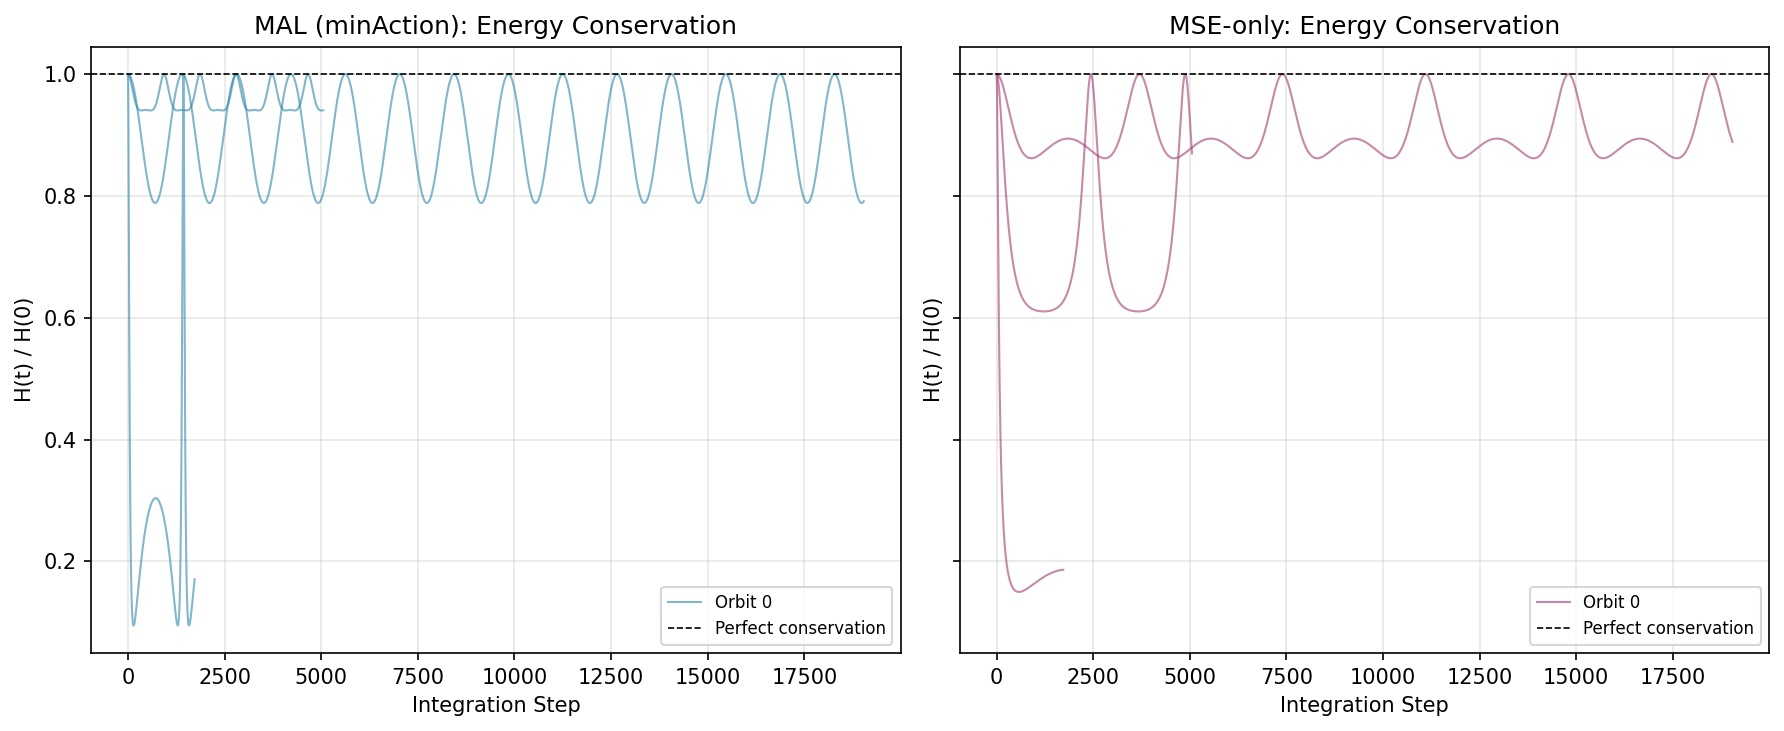
\includegraphics[width=0.45\textwidth]{fig4_energy_conservation.pdf}
\caption{\textbf{Energy-conservation-based model selection and schedule geometry.} (Left) Phase-space trajectory of $(\alpha_E, \tau)$ during training, color-coded by epoch. Red diamonds mark epochs where the ratio $\alpha_E / \tau$ passes through integer values (3:1, 2:1, 1:1), coinciding with major transitions in gate selectivity (onset, sparsification, crystallization). These coincidences arise from the designed schedule geometry; whether they reflect deeper dynamical principles remains an open question (see Discussion). (Right) Energy conservation $\sigma_H$ by selected basis: correct $r^{-2}$ models conserve $H$ over long-horizon rollouts, while incorrect bases violate Hamiltonian dynamics despite matching short-term trajectories. This provides an energy-conservation-based diagnostic for model selection.}
\label{fig:energy}
\end{figure}

\textbf{Schedule geometry and gate transitions.} Analysis of the designed schedule trajectory $(\alpha_E(t), \tau(t))$ reveals that major gate transitions coincide with epochs where the ratio $\alpha_E / \tau$ passes through specific integer and near-integer values: gate onset ($R \geq 10$) near $\alpha_E/\tau \approx 2\text{:}3$, rapid sparsification near $\alpha_E/\tau \approx 1\text{:}1$, and final crystallization ($R \geq 1000$) near $\alpha_E/\tau \approx 2\text{:}1$ (Fig.~\ref{fig:energy}). We emphasize that these coincidences arise from the designed schedule geometry: because $\alpha_E$ ramps linearly and $\tau$ decays exponentially, any smooth trajectory through this parameter space will necessarily pass through integer-ratio nodes (a consequence of the density of rationals). Whether the gate dynamics are genuinely \textit{sensitive} to these passages---as opposed to merely coincident with them---remains an open question requiring perturbation experiments (see Discussion).

\textbf{Architectural sparsification.} The $E_{\mathrm{min}}$-driven soft-to-discrete transition produces near-one-hot gate distributions: gate concentration $C_{\mathrm{gate}} = 0.99 \pm 0.02$ (Herfindahl--Hirschman Index on effective gate contributions $A_i|\theta_i|$; $C_{\mathrm{gate}} = 1$ indicates complete concentration on a single basis) for MAL-trained models ($N=10$ seeds) vs.\ $C_{\mathrm{gate}} = 0.14 \pm 0.04$ for teacher-forcing-only baselines (Mann--Whitney $U = 100$, $p < 10^{-4}$; permutation test $p < 0.001$, $n=10{,}000$; Supplemental Material, Fig.~S6). This architectural sparsification is consistent with Clune \textit{et al.}'s~\cite{Clune2013} finding that minimizing wiring costs---a proxy for metabolic expenditure---produces modular structure in evolved networks.

\textbf{Structural parallels.} The sparse architectures produced by MAL's energy-constrained optimization parallel modular structures observed in networks evolved under wiring-cost pressure~\cite{Clune2013, Bullmore2012}. Whether energy-constrained optimization generically produces similar architectural motifs across biological and artificial systems is a hypothesis warranting formal investigation; we discuss cross-domain parallels further in the Supplemental Material (Sections~S5--S6).

\subsection{Comparison to alternative approaches}
We benchmarked MAL against five alternatives on the Kepler-with-noise problem (Supplemental Material, Section S4, Supplemental Tables~S5--S6):

\textbf{(1) SINDy variants~\cite{Brunton2016, Hirsh2022GPSINDy, Fasel2022EnsembleSINDy}:} Vanilla SINDy with naive differentiation (stride $s=1$) fails completely (noise-dominated). However, when equipped with the same wide-stencil preprocessing ($s=10$) used in MAL, vanilla SINDy identifies $r^{-2}$ in 10/10 seeds, GP-SINDy in 8/10, and ensemble-SINDy in 10/10 (Supplemental Table~S5). \textit{The wide-stencil technique is the critical enabler, not the learning algorithm.} SINDy's advantage is speed ($<1$~s vs.\ $\sim$835~s); its limitation is the absence of dynamical validation---SINDy returns sparse coefficients but cannot roll out trajectories or verify energy conservation. MAL's energy-conservation diagnostic provides this additional layer.

\textbf{(2) HNN~\cite{Greydanus2019} and LNN~\cite{Cranmer2020LNN}:} Trained on identical data (Supplemental Table~S6). HNN (17K parameters, 113~s) achieved excellent energy conservation ($\sigma_H = 4.1 \times 10^{-4}$) but learns a black-box Hamiltonian with no interpretable symbolic form. LNN (17K parameters, 242~s) suffered from Hessian singularities, with validation loss diverging to $10^6$ throughout training---a known failure mode for LNNs on noisy data where the mass matrix becomes ill-conditioned. Neither method performs basis selection or yields a symbolic force law.

\textbf{(3) Mathematical LLM (Qwen2-Math 7B):} 0\% on inverse problems, 61\% on forward derivation (Supplemental Material, Section~S1).

\textbf{(4) Physics-informed NN~\cite{Raissi2019}:} 85\% when the inverse-square law is pre-specified, but cannot identify the law \textit{de novo}.

\textbf{(5) Teacher-forcing only (no $\mathcal{L}_{E_{\min}}$):} Gates remained at 45\% (failed to crystallize); energy consumption 77\% higher.

\textbf{Summary of niche.} MAL occupies a distinct position: it combines interpretable symbolic basis selection (shared with SINDy~\cite{Brunton2016}) with dynamical rollout and energy-conservation validation (shared with HNN~\cite{Greydanus2019}), while adding explicit sparsity-driven efficiency optimization. HNNs/LNNs~\cite{Greydanus2019, Cranmer2020LNN} guarantee conservation but produce black-box energy functions; SINDy~\cite{Brunton2016} yields symbolic expressions but without dynamical consistency checks; MAL provides both within an energy-constrained framework.

\section{Discussion}

\subsection{Key findings}
Our results establish four principal findings:

\textbf{(1) Sparsity constraints improve physical law identification.} Embedding energy minimization ($E_{\min}$) alongside information maximization ($I_{\max}$) in the triple-action training objective constrains the model selection problem from an unconstrained search to a tractable optimization. The $E_{\mathrm{min}}$ subsystem drives gate crystallization (basis selection) that does not occur under prediction error alone, while reducing training energy by 40\%.

\textbf{(2) Wide-stencil preprocessing enables identification; MAL adds dynamical validation.} Our comparison with SINDy variants (Supplemental Material, Table~S5) reveals that wide-stencil preprocessing ($s=10$) is the critical enabler for \textit{all} methods, including vanilla SINDy (10/10 correct identification). This transparency is important: SINDy achieves comparable basis selection at $<1$\% of MAL's computational cost. However, SINDy returns sparse coefficients without dynamical consistency checks---it cannot roll out trajectories, verify energy conservation over multiple orbital periods, or detect when a numerically adequate fit corresponds to incorrect physics. MAL's energy-conservation model selection criterion (Supplemental Material, Table~S2) fills this gap: models selecting incorrect bases ($r^{-1}$, $r^{-3}$) produce comparable short-term trajectory accuracy but violate Hamiltonian conservation by $3$--$6\times$, revealing their failure to capture the true causal structure. We note that a similar check could in principle be applied post-hoc to SINDy output. MAL's advantage lies in end-to-end differentiability---the conservation criterion participates in training, not just post-hoc evaluation---and in extensibility to systems where SINDy's linear regression may fail (e.g., problems with latent variables or non-separable coupling). Demonstrating this advantage on such systems is an important direction for future work.

\textbf{(3) Intrinsic crystallization timescales.} The gate competition dynamics exhibit universal timescales: crystallization span $\Delta t_{\text{span}} = 36.2 \pm 4.1$ epochs and geometric growth rate $\gamma = 1.137 \pm 0.013$ per epoch, independent of which basis wins or the initialization seed. We also observe that major gate transitions coincide with epochs where the schedule ratio $\alpha_E / \tau$ passes through integer values, though this may simply reflect the density of rationals along any smooth trajectory through parameter space. Whether the crystallization dynamics are genuinely sensitive to these passages requires perturbation experiments, which we leave to future work.

\textbf{(4) Architectural sparsification from energy minimization.} Clune \textit{et al.}~\cite{Clune2013} demonstrated that networks evolving under pressure to minimize connection costs spontaneously develop modular architectures. Our work shows a related pattern: MAL's sparse gate selection ($C_{\mathrm{gate}} = 0.99$) emerges from $\mathcal{L}_{E_{\min}}$ without a pre-programmed bias toward any particular basis. This supports the broader principle that cost-constrained optimization drives architectural sparsification in both biological~\cite{Bullmore2012} and artificial systems.

\subsection{Broader implications}
\textbf{Energy-efficient scientific machine learning.} MAL's 40\% energy reduction over prediction-error-only baselines demonstrates that explicit sparsity constraints can improve computational efficiency without sacrificing task performance. The mechanism is architectural: $\mathcal{L}_{E_{\min}}$ drives early gate crystallization, reducing the effective parameter count and shortening convergence. This principle---that sparsity-inducing regularization simultaneously improves interpretability and efficiency---may generalize to larger-scale scientific discovery tasks.

\textbf{Noether-based model selection.} A persistent challenge in scientific machine learning is distinguishing genuine physical understanding from statistical correlation~\cite{Pearl2019}. The energy-conservation criterion---preferring models that preserve Hamiltonian dynamics over long-horizon rollouts---provides a physics-grounded approach complementary to recent work on learning conserved quantities~\cite{vanderOuderaa2024, Tanaka2021}. Models that violate energy conservation reveal their failure to capture true causal structure, even when matching short-term predictions.

\subsection{Limitations and future directions}
\textbf{Fixed basis library.} MAL requires pre-specifying candidate force laws $\{\phi_i\}$, with the correct answer included. This makes MAL a model \textit{selection} framework, not an open-ended \textit{discovery} system. Basis library sensitivity experiments (Supplemental Material, Section S4F) quantify this limitation: adding near-confounders ($r^{-2.5}$, $r^{-1.5}$) reduces the correct-basis rate from 50\% to 20\%, while removing the correct basis ($r^{-2}$) causes the system to split between alternatives. Distant additions ($r^2$, $r^{-4}$, $\ln r$) have no effect. In all cases, the energy-conservation diagnostic remains informative, and uniformly elevated $\sigma_H$ across seeds flags potential library inadequacy. Extending to genuinely autonomous discovery---where the algorithm constructs novel functional forms not in the library---requires integration with open-ended symbolic regression methods \cite{Udrescu2020, Cranmer2020} or LLM-guided symbolic search, which is an important direction for future work.

\textbf{Two benchmarks, limited scope.} We have validated MAL on two central-force problems (Kepler and Hooke) in 2D with synthetic data. The generality of our claims would be substantially strengthened by additional benchmarks: non-central forces (e.g., magnetic fields), dissipative systems (e.g., damped oscillators), higher dimensions, coupled multi-body problems, and semi-real data (e.g., planetary ephemerides with actual measurement noise). The core principle---embedding action minimization in differentiable networks---should transfer, but this remains to be demonstrated.

\textbf{Correct-basis success rate.} Without logit initialization, only 4 of 10 Kepler seeds directly select $r^{-2}$, necessitating cross-seed application of the energy-conservation-based diagnostic. Biased initialization resolves this (10/10), but requires prior knowledge of which basis to favor. Understanding the logit-gradient dynamics that determine gate competition---and developing initialization-free methods to improve the raw success rate---remain priorities.

\section{Conclusion}
We have demonstrated that minimum-action learning---neural network training guided by a triple-action functional combining information maximization, energy minimization, and symmetry enforcement---enables energy-constrained identification of physical force laws from noisy data. Validated on two benchmarks (Kepler gravity and Hooke's linear restoring force), the key technical contributions are: (1)~the wide-stencil noise reduction technique that transforms an intractable problem (SNR~$\sim 0.02$) into a learnable one (SNR~$\sim 1.6$); (2)~the soft-to-discrete gate sharpening mechanism that achieves basis selection through energy-driven architectural crystallization, with a physics-informed initialization achieving 10/10 correct selection; and (3)~the energy-conservation-based model selection criterion that discriminates correct from incorrect physics via long-horizon Hamiltonian conservation. Direct comparison against SINDy variants, HNNs, and LNNs confirms MAL's distinct niche: interpretable, energy-constrained model selection combining symbolic basis identification with dynamical validation.

Future work will extend MAL to non-central forces, dissipative systems, higher-dimensional problems, and real observational data (e.g., planetary ephemerides), and will test whether the intrinsic crystallization timescales and schedule-geometry coincidences observed here generalize across problem classes.

\section{Methods}
\label{sec:methods}

\subsection{Data generation}
We simulated $N=16$ Keplerian orbits in 2D using a symplectic velocity-Verlet integrator with gravitational units $G = M = 1$. Semi-major axes $a$ were sampled log-uniformly over $[0.5, 5.0]$~AU; eccentricities $e$ uniformly over $[0, 0.3]$. Each orbit was integrated for 5 orbital periods at timestep $\Delta t_{\text{sim}} = 10^{-3}$, then downsampled to observation cadence $\Delta t_{\text{obs}} = 0.05$. Gaussian noise $\mathcal{N}(0, \sigma^2)$ with $\sigma = 0.01 \times \text{median}(a)$ was added to all position measurements. Data were split 70/15/15 into training, validation, and test sets.

\subsection{Neural architecture}
\textbf{Noether Force Basis.} The force module computes:
\begin{equation}
\mathbf{F}(\mathbf{r}) = -\left[\sum_{i=1}^5 A_i \theta_i \phi_i(r)\right] \frac{\mathbf{r}}{r}
\end{equation}
where $\phi_i \in \{r^{-2}, r^{-1}, r, 1, r^{-3}\}$, $\theta_i$ are learnable scalars (force magnitudes), and $A_i = \mathrm{softmax}(\ell_i / \tau)$ are gates with logits $\ell_i$ and temperature $\tau$. SO(2) symmetry is enforced by restricting dependence to radial distance $r = |\mathbf{r}|$. Candidate basis functions are treated as phenomenological radial scalings; dimensional consistency resides in the fitted coefficients $\theta_i$ rather than in the basis library itself.

\textbf{MinActionNet Integrator.} The selected force law is embedded in a velocity-Verlet integrator:
\begin{align}
\mathbf{v}_{1/2} &= \mathbf{v}_n + \tfrac{\Delta t}{2} \mathbf{F}(\mathbf{r}_n), \nonumber \\
\mathbf{r}_{n+1} &= \mathbf{r}_n + \Delta t \, \mathbf{v}_{1/2}, \\
\mathbf{v}_{n+1} &= \mathbf{v}_{1/2} + \tfrac{\Delta t}{2} \mathbf{F}(\mathbf{r}_{n+1}), \nonumber
\end{align}
with model timestep $\Delta t_{\text{model}} = \Delta t_{\text{obs}} / 5 = 0.01$ to ensure numerical stability while maintaining computational efficiency.

\subsection{Loss function}
The triple-action functional (Eq.~\ref{eq:triple-action}) decomposes as:

\textbf{Information term} ($\mathcal{L}_{I_{\max}}$):
\begin{align}
\mathcal{L}_{\text{traj}} &= \frac{1}{T-1} \sum_{k=0}^{T-2} \|\mathbf{r}_{\text{pred}}(t_{k+1}) - \mathbf{r}_{\text{obs}}(t_{k+1})\|^2, \\
\mathcal{L}_{\text{accel}} &= \frac{1}{T-2s} \sum_{j=s}^{T-s-1} \|\mathbf{F}_{\text{model}}(\mathbf{r}_j) - \hat{\mathbf{a}}_j\|^2,
\end{align}
where $\hat{\mathbf{a}}_j = (\mathbf{r}_{j+s} - 2\mathbf{r}_j + \mathbf{r}_{j-s}) / (s \Delta t)^2$ is the wide-stencil acceleration estimate with stride $s=10$, and $\mathcal{L}_{I_{\max}} = \mathcal{L}_{\text{traj}} + \lambda_{\text{accel}} \mathcal{L}_{\text{accel}}$ with $\lambda_{\text{accel}} = 1.0$.

\textbf{Energy term} ($\mathcal{L}_{E_{\min}}$):
\begin{align}
\mathcal{L}_{\text{sym}} &= \text{Var}[E(\mathbf{r}_k, \mathbf{v}_k)] = \langle (E - \langle E \rangle)^2 \rangle, \\
\mathcal{L}_{\text{comp}} &= \langle |A_i \theta_i| \rangle_i, \\
\mathcal{L}_{\text{arch}} &= -\sum_{i=1}^5 A_i \log A_i,
\end{align}
where $E = \tfrac{1}{2}|\mathbf{v}|^2 - GM/r$ is the orbital energy, $\mathcal{L}_{\text{comp}}$ is the scale-invariant sparsity penalty, $\mathcal{L}_{\text{arch}}$ is the gate entropy, and $\mathcal{L}_{E_{\min}} = \mathcal{L}_{\text{sym}} + \lambda_{\text{comp}} \mathcal{L}_{\text{comp}} + \lambda_{\text{arch}} \mathcal{L}_{\text{arch}}$ with $\lambda_{\text{comp}} = 0.01$, $\lambda_{\text{arch}} = 0.5$.

\subsection{Training protocol}
\textbf{Two-phase schedule:}
\begin{itemize}
\item \textit{Phase 1 (Warmup, epochs 1--50):} $\alpha_I = 1.0$, $\alpha_E = 0.01$, $\tau = 1.0$. Low regularization allows gates to explore gradient signal from $\mathcal{L}_{\text{accel}}$.
\item \textit{Phase 2 (Sparsification, epochs 51--200):} $\alpha_I = 1.0$, $\alpha_E$ ramps linearly $0.01 \to 1.0$, $\tau$ decays exponentially $1.0 \to 0.05$. Increasing $\alpha_E$ drives gate competition; decreasing $\tau$ sharpens softmax toward one-hot.
\end{itemize}

\textbf{Optimizer:} Adam with learning rate $10^{-3}$, batch size 4, training for 200 epochs on an NVIDIA RTX 2080 Ti GPU.

\textbf{Post-training calibration:} After gate convergence, the L1 penalty has biased $\theta_i$ toward zero. We correct via least-squares projection:
\begin{equation}
\theta_{\text{opt}} = \frac{\sum_j \phi_{\text{dom}}(r_j) \hat{a}_{\text{radial},j}}{\sum_j \phi_{\text{dom}}(r_j)^2},
\end{equation}
where $\phi_{\text{dom}}$ is the dominant basis function, $\hat{a}_{\text{radial},j} = -\hat{\mathbf{a}}_{\text{wide},j} \cdot \hat{\mathbf{r}}_j$ are radial projections of the wide-stencil acceleration estimates $\hat{\mathbf{a}}_{\text{wide}}$ (defined in Eq.~5 with stride $s=10$), and sums run over all training midpoints $j \in [s, T-s-1]$.

\subsection{Validation metrics}
\textbf{Kepler exponent:} Orbital periods $T_i$ were estimated from test-set trajectories via autocorrelation peak detection with proper normalization by overlapping sample count. Power-law regression $T^2 = C a^p$ yielded $\hat{p}$ and $\hat{C}$.

\textbf{Energy conservation:} For long-horizon rollouts (5 orbital periods from test-set initial conditions, using the velocity-Verlet integrator at $\Delta t_{\text{model}} = 0.01$ with the post-calibration coefficient $\theta_{\text{opt}}$), we computed Hamiltonian variance $\sigma_H^2 = \langle (H - \langle H \rangle)^2 \rangle$ as an energy-conservation diagnostic: correct force laws preserve $H$; incorrect laws violate conservation despite matching short-term trajectories.

\textbf{Gate concentration:} Architectural sparsification was quantified via the Herfindahl--Hirschman Index (HHI) on effective gate contributions $p_i = A_i|\theta_i| / \sum_j A_j|\theta_j|$, yielding $C_{\mathrm{gate}} = (K \cdot \text{HHI} - 1)/(K-1) \in [0,1]$ where $K=5$ basis functions. $C_{\mathrm{gate}}=1$ indicates complete concentration on a single basis; $C_{\mathrm{gate}}=0$ indicates uniform distribution.

\subsection{Code and data availability}
All code, trained models, and synthetic data are available at \url{https://github.com/martinfrasch/minAction_kepler}. Experiments were implemented in PyTorch 2.0 on Python 3.10.

\begin{acknowledgments}
I thank my family for giving me space to follow my ideas.
\end{acknowledgments}

\bibliography{references}

\end{document}
